\chapter{Background} \label{chapter:BACKGROUND}

Our approach, as described in Chapter~\ref{chapter:APPROACH}, provides object versioning for prototype-based programming systems.
Prototype-based programming uses objects as building blocks for applications.
One particular example of such a system is Lively, a self-supporting web-based programming system with tools to directly edit graphical objects.
Lively is also the system for which we implemented our approach.

A key motivation for our approach is CoExist.
CoExist applies continuous versioning to provide recovery support automatically: programmers have access to a fine-grained history of development states without having to take any explicit precautionary actions themselves.

\section{Prototype-based Programming}

Prototype-based programming is object-oriented programming, in which applications are constructed using only objects, without classes.
Examples for programming languages or systems that implement prototype-based programming are Self, JavaScript, and Kevo~\cite{Taivalsaari1992Kevo}.
Self and JavaScript incorporate prototypical inheritance.
They allow objects to inherit state and behavior directly from other objects: an object has a prototype to which it delegates when looking up a property in the object itself yields no results.
Kevo, in constrast, does not provide this kind of delegation, but allows to make full copies of objects.
Programmers can create new objects with initially the same state and behavior as existing ones, but all objects remain self-contained.
That is, in Kevo, changing an object only changes that particular object and a particular object can only be changed by directly changing it, not by, for example, changing a prototype or a class.

Despite this difference, prototype-based programming allows to build programs by creating particular objects, in contrast to the class-based style of object-oriented programming, in which programs are defined in abstract structure and behavior descriptions.
In particular, each of the parts of a program is an object with particular state, a particular example instead of a general category.

There are different advantages associated with this kind of programming:
\begin{itemize}
    \item \cite{Taivalsaari1996CVP} and \cite{Ungar1987SPS} argue that developers may easier understand concrete examples than abstract classes of objects. A concrete example provides particular values for its states and, in case of objects with a visual appearance, can be actually looked at.
    \item \cite{Ungar1987SPS} and \cite{Borning1986CVP} describe how prototype-based programming makes it easier to introduce one-of-a-kind objects with their own structure or behavior.
    \item \cite{Borning1986CVP} and \cite{Maloney1995Mor} make the point that especially programming visual elements can be more concrete with prototypes. Instead of writing code to define the appearance of objects, developers can manipulate particular graphical elements directly. Developers could, for example, use the mouse to manipulate properties like the size, position, and style or to combine multiple basic elements into one composition. This way, developers always see intermediate states and do not only receive feedback on explicit test runs in-between edit-compile-load cycles or run/edit distinctions. 
\end{itemize}

Similarly to the previous examples, many end-user programming systems, including Scratch\cite{Maloney2010SPL}, Etoys~\cite{Kay2005Etoys}, or Fabrik~\cite{Ingalls1988FVP}, enable users to express their programs in particular objects, all with graphic representations and tools to directly manipulate those.
In addition, programmers manipulate objects at runtime in these end-user programming systems and many general-purpose prototype-based programming systems, like Lively, Self, and Kevo.
These also provide tools for manipulating graphical objects directly, where graphical elements range from simple objects like primitive shapes over interactive widgets to applications that are more directly useful like presentation software or programming tools.
In general, development at runtime, prototype-based programming, and direct manipulation of graphical elements seem properties of programming systems that suit each other.



\section{The Lively Kernel}

Lively, also referred to as the \emph{Lively Kernel}, is a browser-based programming system in the tradition of both Smalltalk and Self.
It incorporates tools and techniques to be completely self-sufficient.
Development in Lively happens at runtime, and programmers can create and save new version of the Lively Kernel itself.

Lively is based in the JavaScript programming language.
Therefore, the system and applications are expressed in a prototype-based object-oriented language that also provides prototypical inheritance.
At the same time, Lively also provides a class system for JavaScript and considerable parts of the system itself are expressed using classes.
One of these parts expressed through classes is an implementation of Morphic~\cite{Maloney1995Mor}, a framework for developing graphical applications.
Programmers can alter graphical objects of this framework, which are called \emph{Morphs}, using direct manipulation and through a number of tools.

\begin{figure}[h]
    \centering
    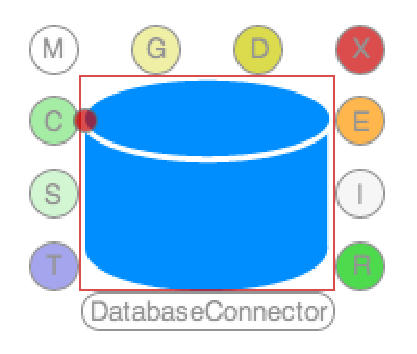
\includegraphics[width=0.3\textwidth]{figures/halos.pdf}
    \caption{The halo buttons of a simple morph.}
    \label{fig:Halos}
\end{figure}

Programmers can change the position of morph objects by dragging and the composition by an alternative dragging, which is called \emph{grabbing}.
A composition of morphs is also contained in a morph---a morph with submorphs---and this way, morphs are not limited to to be basic shapes or simple widgets, but can be the entire user interface of arbitrary applications.
Lively further provides a set of manipulation tools, called \emph{Halos}, as shown in Figure~\ref{fig:Halos}, that developers can bring up directly at morphs.
The different halo buttons allow, for example, to resize~\textcircled{R}, rotate~\textcircled{T}, and copy~\textcircled{C} morphs.
The copy operation does not establish a prototypical inheritance relationship between the copy and the original, but copies entire state, including of which class the copy is an instance.
Other halo buttons open specific tools, which are shown in Figure~\ref{fig:LivelyTools} to further manipulate the morphs:

\begin{enumerate}
    \item The \emph{Inspector}~\textcircled{1} presents all the values that make up a morph's state. It also has a small code pane at the bottom, intended to be used to manipulate the state programmatically.
    \item The \emph{Style Editor}~\textcircled{2} allows to manipulate certain aspects of a morph's visual appearance. Programmers can use it to, for example, change a morphs color, border width, or the layout of its submorphs.
    \item The \emph{Object Editor}~\textcircled{3} is a tool dedicated to the object-specific behavior of morphs, which are called \emph{scripts} in Lively. It shows all scripts of a particular morph, but also can add and adapt scripts to that.
\end{enumerate}

\begin{figure}[h]
    \centering
    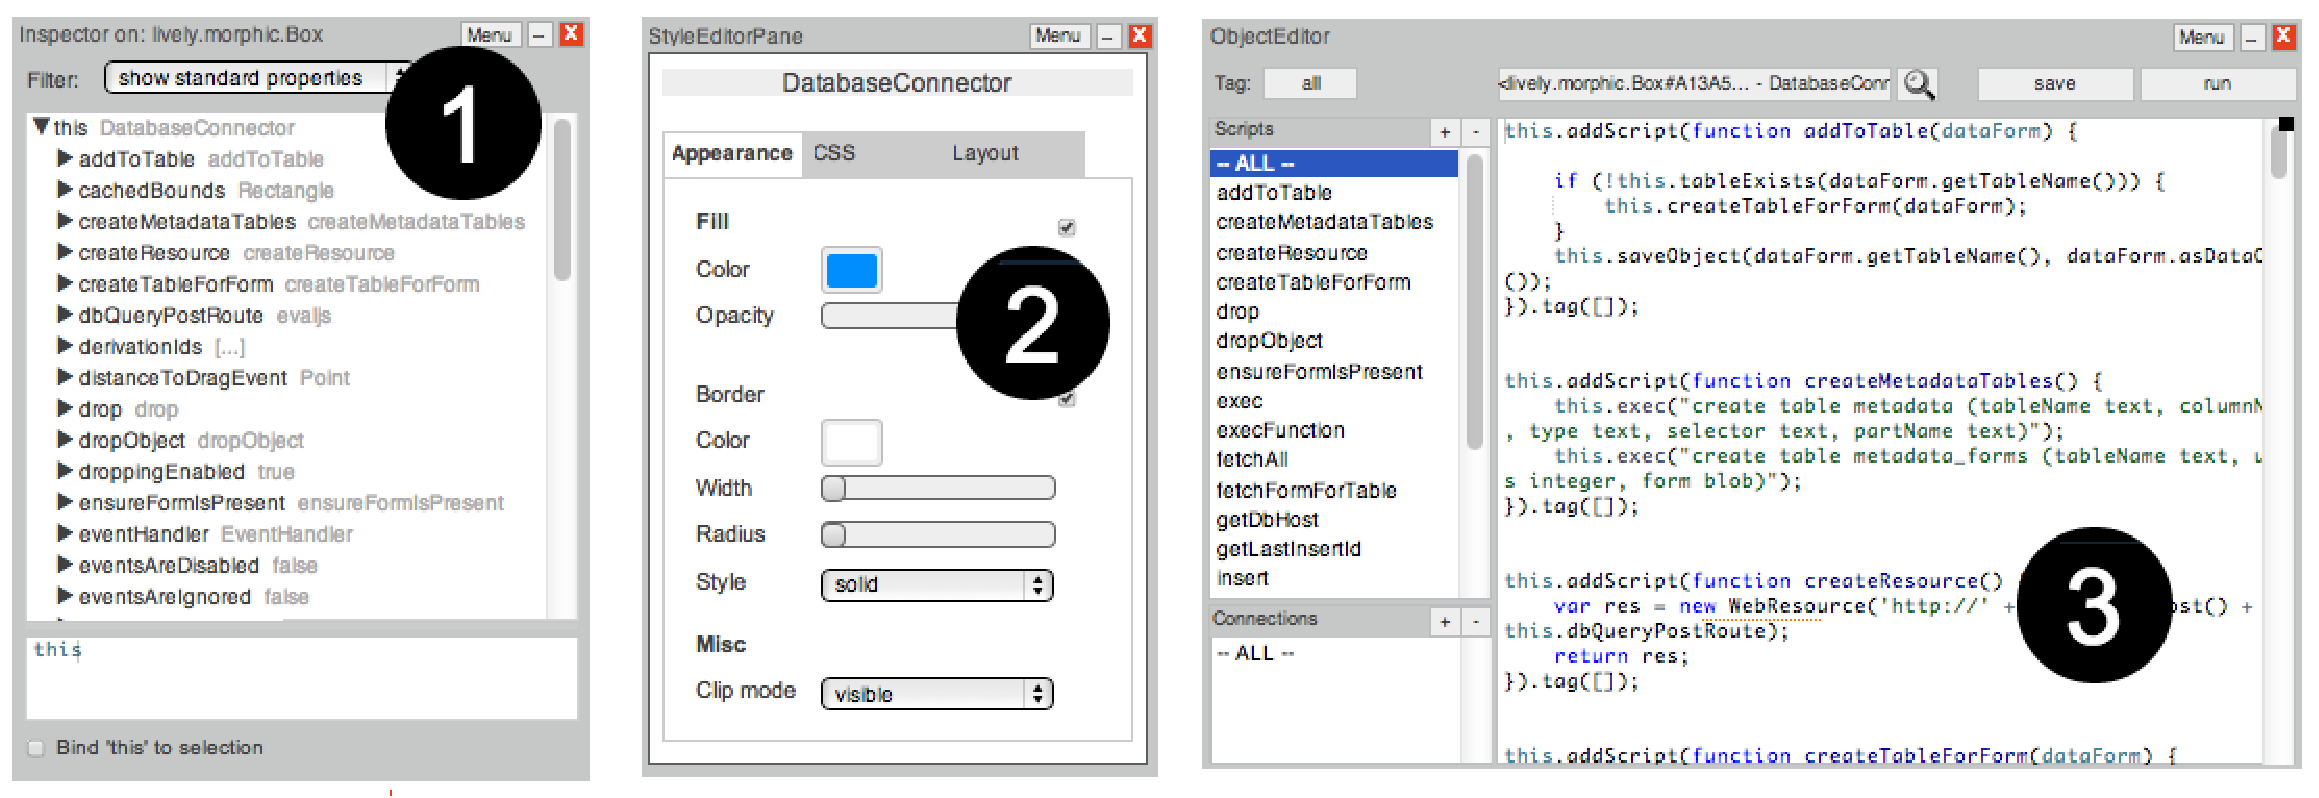
\includegraphics[width=\textwidth]{figures/livelyTools.pdf}
    \caption{Lively's tools to manipulate properties of morphs, from left to right: the Inspector, the Style Editor, and the Object Editor.}
    \label{fig:LivelyTools}
\end{figure}

\begin{figure}[h]
    \centering
    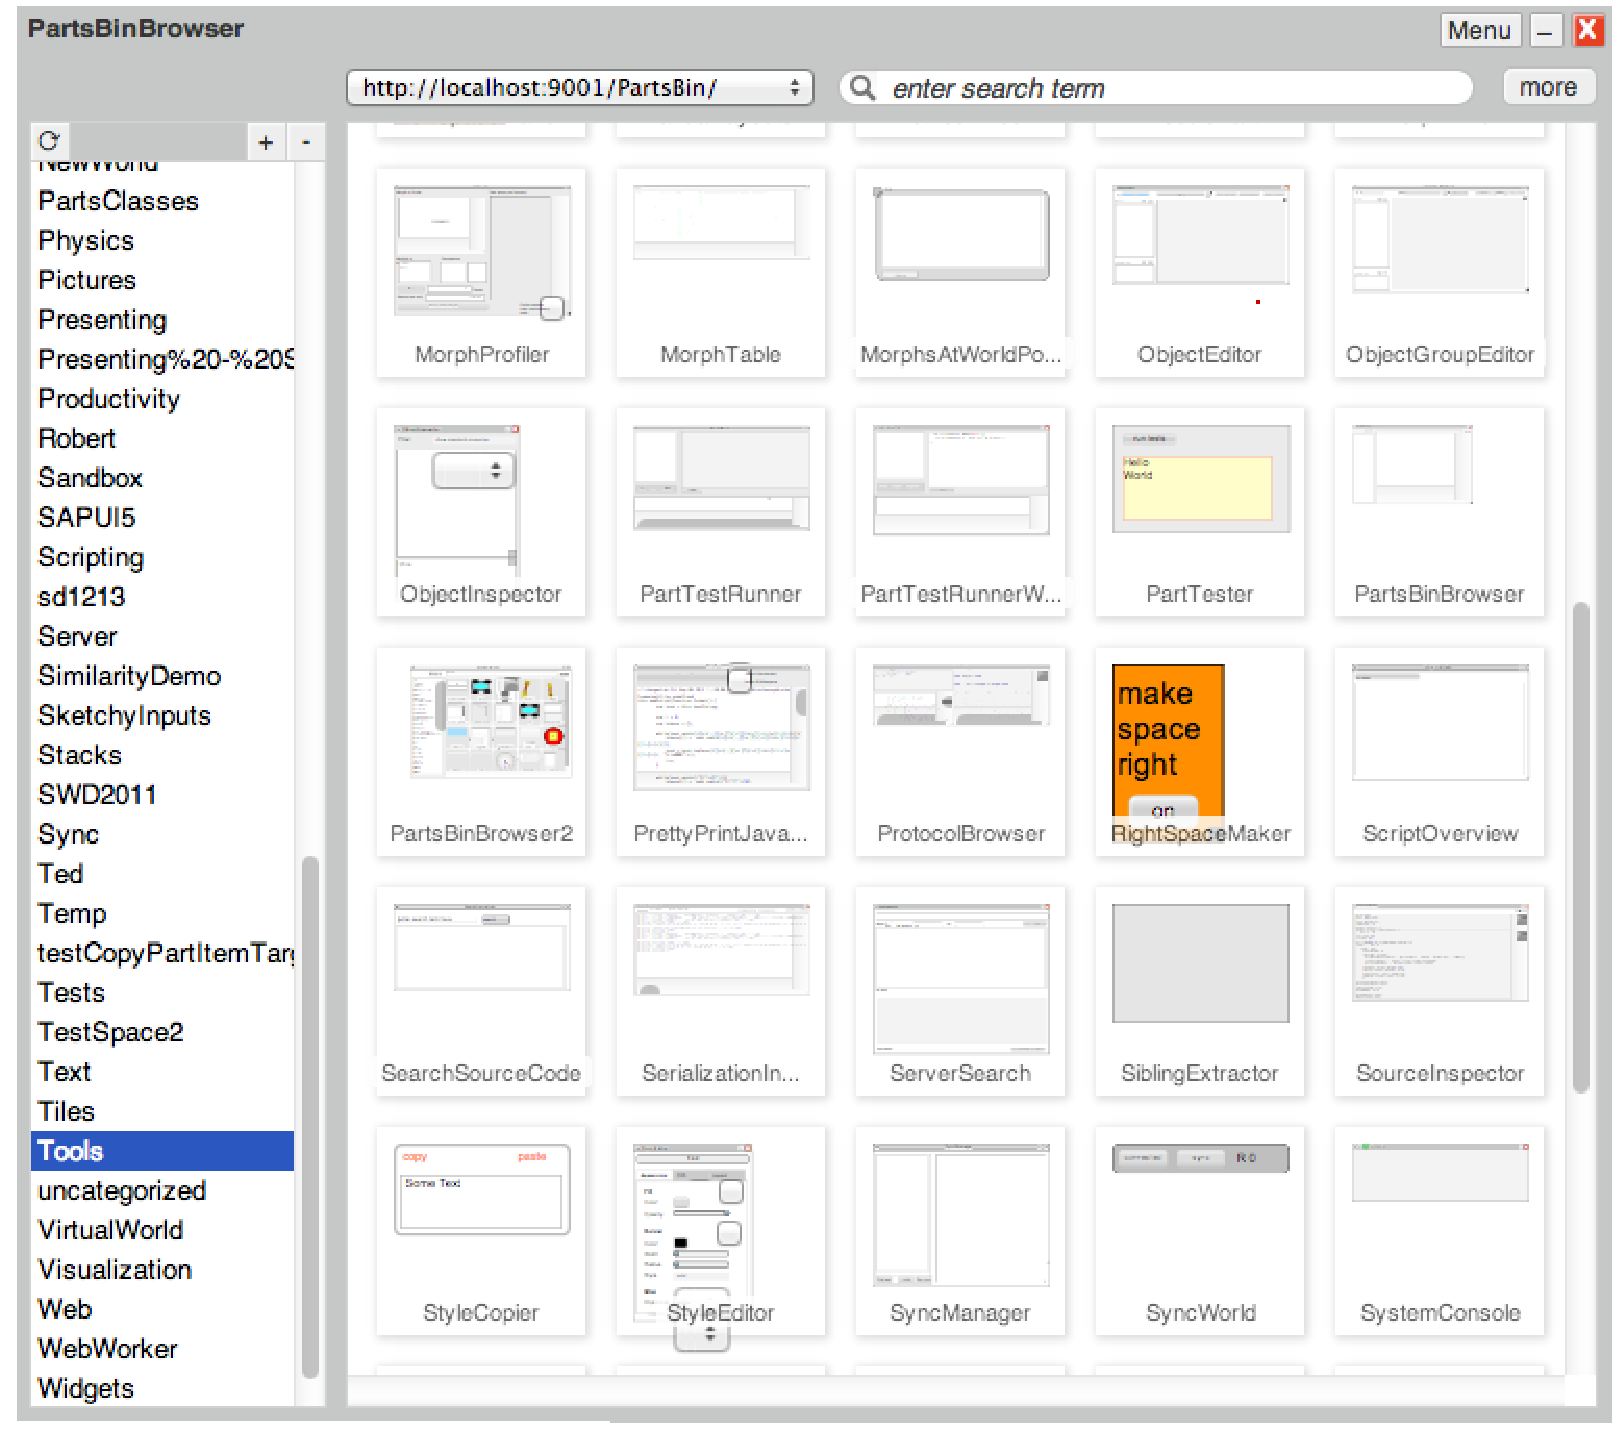
\includegraphics[width=0.7\textwidth]{figures/partsBin.pdf}
    \caption{Lively's Parts Bin opened on the \emph{Tools} category.}
    \label{fig:PartsBin}
\end{figure}

Another tool related to morphs, though not available from a halo button, is Lively's \emph{Parts Bin}~\cite{Lincke2012LPC}, an object repository to save and load specific versions of morphs.
Morphs saved to the Parts Bin are called \emph{parts} to emphasize the ability to reuse any one of the morphic implementations stored in the Parts Bin in another application.
Figure~\ref{fig:PartsBin} shows the Parts Bin and, in particular, a group of tools that the Parts Bin contains, which also includes both the Style Editor and the Object Editor.
Both these tools are examples for graphical applications developed from available parts, with their logic expressed in scripts, and saved to the Parts Bin.



\section{CoExist}

CoExist\footnote{\url{http://www.bastiansteinert.org/coexist.html}, accessed February 28, 2014} supports programmers through automatic and continuous versioning.
The IDE extension preserves each indermediate development state with its respective source code and associated runtime information.
The states are recorded as separate version in their original order and along with change summaries, associated test results, and screenshots of the development environment.
Programmers can review their development sessions, inspect the impact each individual change had on test cases, and recover previous development states.
They can completely withdraw withdraw changes or only re-visit a previous state to recover information as, for example, the source code for a specific method.

\begin{figure}[h]
    \centering
    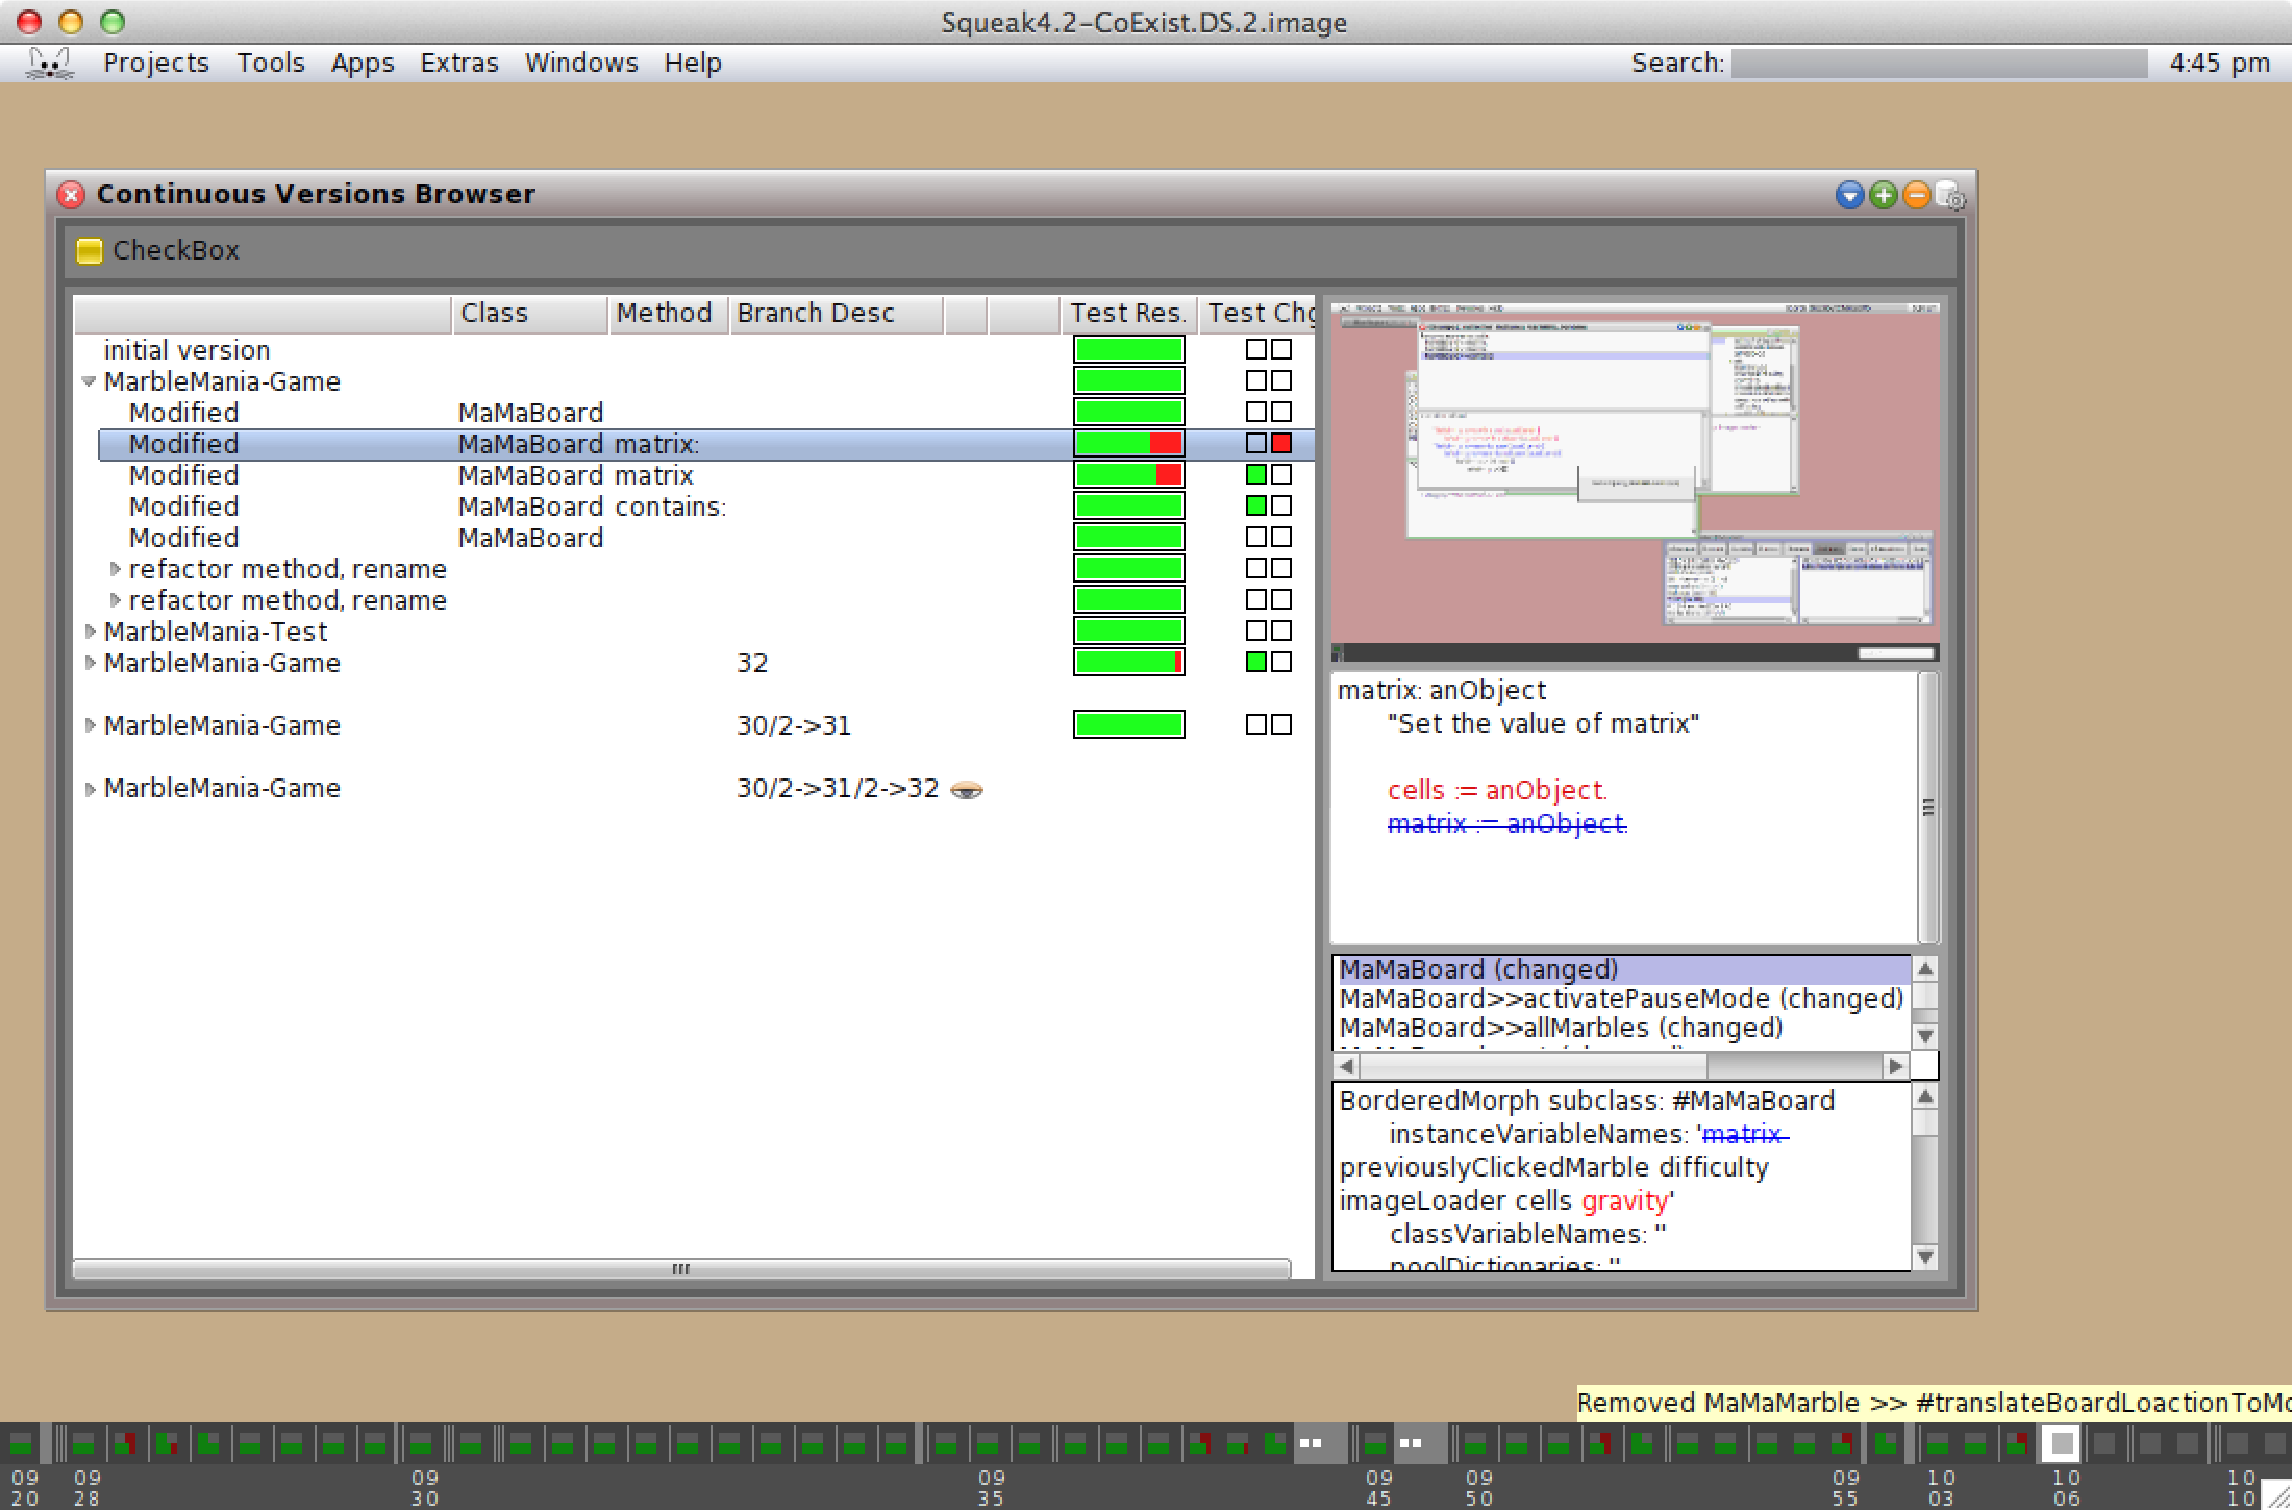
\includegraphics[width=0.7\textwidth]{figures/coexistTools.pdf}
    \caption{CoExist's tools to manage the preserved development states: a timeline and a Version Browser.}
    \label{fig:CoExist}
\end{figure}

CoExist provides tools to help programmers benefit from the preserved development histories, shown in Figure~\ref{fig:CoExist}.
CoExist adds a timeline tool to the bottom of the development environment.
It presents each intermediate version through a small rectangle that indicates the impact on test cases: the bottom of the rectangle shows how many test cases passed and failed totally, while the top half highlights only test results that changed for this version.
Hovering above such a version rectangle also indicates what has changed---which method of which class.
Clicking a version provides access to its source code and more information on test results, but also allows to re-establish the version.
Besides this timeline of all changes, a Version Browser tool shows changes to different modules separately.
It presents the same information on test cases, but in addition offers diffs and how the development environment appeared in each version.
The two tools support programmers in re-tracing their steps, understanding the impact of their actions in retrospect, and in recovering information from previous development states.

This way, CoExist is intented to reduce the effort that programmers usually put into recovery, either into actual compensational actions or into precautionary actions.
To re-establish a previous development state---because of, for example, unintentionally introduced errors, decreased performance, or harmed design---programmers can manually repair improperly changed code or load a previously commited version of the sources.
Programmers can preserve specific versions to be able to easily withdraw changes, and, thus, reduce the cost of recovery by anticipating recovery needs beforehand.
However, preserving versions manually is also an effort and especially so when revision histories are expected to be well-documented and immediately useful.
For that, programmers need to assemble changes to meaningful increments, test these, and write version descriptions.
Testing each one directly also helps to find introduced problems early on intead of analyzing longer lists of changes that all could have introduced a problem.

With CoExist, developers do not have to take explicit precautionary actions, but still have access to a fine-grained history of development states and even to test results for each individual state.
This is intended to encourage programmers to try ideas without worrying about negative consequences.
They can focus on implementing new ideas and their actual programming tasks, and rely on CoExist to help in case any action unexpectedly needs to be undone.


\todo{Structured: not just like auto-save (google docs), but structured: associated with particular actions and the static structure of programs... class>>method (add/delete/modify).. and also cross-document}


% In contrast to having developers manually preserve particular versions of their code and run the appropriate set of test cases for such, CoExist provides automatic recovery support.
% Every change made to source code yields a version for which CoExist also captures test results and a screenshot of the development state.
% Thus, developers have access to a fine-grained and rich history of development states when they need to recover previous situations.
% 
% CoExist allows developers to recover previous versions of the code without having to take precautionary actions manually.
% For each of those versions CoExists then automatically also captures test results and screenshots of the development environment, helping developers in finding relevant versions when recovery is necessary.
% 
% % Developers do not have to manually create commits or run tests for development states that seem important.
% 
% % sometimes easier to make the changes and experience the results than to anticipate the changes beforehand...)… 
% automatic and continuous versioning of the system code whenever code changes, whenever a user interacts/saves/changes code.
% allows to concentrate on implementing ideas… while a fine-grained versioning history, which can also be enriched with test results and screenshots to support finding relevant versions, is there for every change that turns out inappropriate.. programmers can always just make changes and concentrate fully on implementing them without too much thought and effort going into precautionary actions… because the coexist tool / tool support records all changes and their effect on test case outcomes… 



% This is supposed to reduce both the time spent on and the errors made in manually precautionary actions.
% Without CoExist, developers explicitly save explicit versions of the code and write short summaries, often in form of commit messages.
% Developers also run tests to understand the impact of their changes.
% While running all tests of the system can take a long time, deciding which takes are helpful in evaluating the recent changes also is often a difficult decision.
% As those two tasks are, thus, cumbersome, developers often do not do both for every single change, but aim to save interesting versions, creating a new version for every meaningful increment.
% However, estimating which changes might be risky and, thus, 
% 
% planning and deciding which groups of changes also pose an effort to developers, who need to estimate which 

% motivation for CoExist: explicit precautionary actions like saving versions is laborious and/or error-prone. saving each intermediate version is not practical (writing up some version comment, running all necessary tests, in the case of lively saving all objects takes a moment, often also no distinction between a private temporary snapshot and a meaningful increment that’s to be published and shared), while saving particular important versions is error-prone (not clear which version to save, risk assessment very difficult… reasons for recovery needs mostly unanticipated… recovery often necessary because of a mistake, because something wasn’t considered or anticipated… this risk assessment whether a change will be an actual increment is difficult… 
